\subsection{Szegélyek}

%32
\begin{frame}
  A szegélyeknek állítható a
  \begin{itemize}
    \item stílusa (\texttt{border-style}),
    \item szélessége (\texttt{border-width}), és a 
    \item színe (\texttt{border-color}).
  \end{itemize}
  Megjegyzések:
  \begin{itemize}
    \item Utóbbi kettő csak a stílus beállítása esetén működik.
    \item Minden paraméter állítható külön az egyes oldalakra is.
  \end{itemize}
\end{frame}

%33
\begin{frame}
  \begin{exampleblock}{\textattachfile{szegelyek.html}{szegelyek.html}}
    \scriptsize
    \lstinputlisting[style=HTML,linerange={14-17},numbers=left,firstnumber=14]{szegelyek.html}
  \end{exampleblock}
  \begin{columns}[T]
    \column{0.25\textwidth}
      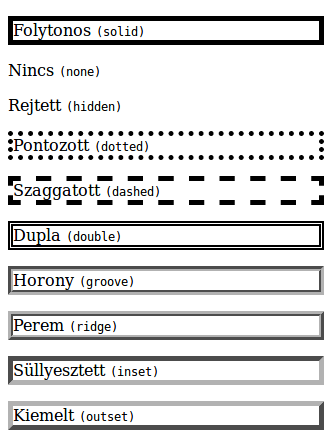
\includegraphics[scale=0.25]{szegelyek.png}
    \column{0.7\textwidth}
      Oldalankénti szegélystílusok megadhatók:
      \begin{itemize}
        \item 1-4 érték megadásával, pl. \\ \texttt{border-style: dotted dashed solid none;}
        \item Oldalakra vonatkozó tulajdonságokkal: 
        \texttt{border-*-style}, ahol \texttt{*} helyén állhat 
        \texttt{top}, \texttt{right}, \texttt{bottom}, \texttt{left}.
      \end{itemize}
  \end{columns} 
\end{frame}

%34
\begin{frame}
  Ha a \texttt{boder-style}-nak
  \begin{description}[m]
    \item[1 értéke van] \hfill \\ \texttt{felül-jobb-alul-bal} (minden 
    oldalra ugyanazt a stílust állítja)
    \item[2 értéke van] \hfill \\ \texttt{felül-alul jobb-bal}
    \item[3 értéke van] \hfill \\ \texttt{felül jobb-bal alul}
    \item[4 értéke van] \hfill \\ \texttt{felül jobb alul bal} (óramutató 
    járása szerint)
  \end{description}
  \vfill
  Hasonlóképpen lehet oldalanként szabályozni a margókat és 
  kitöltéseket is.
\end{frame}

% hidden, none különbség
